\documentclass[12pt,a4paper]{article}

\usepackage[utf8]{inputenc}
\usepackage[english]{babel}
\usepackage{amsmath}
\usepackage{amsfonts}
\usepackage{amssymb}
\usepackage{graphicx}
\usepackage{lmodern}
\usepackage[left=2cm,right=2cm,top=2cm,bottom=2cm]{geometry}

\usepackage{siunitx}
\usepackage{enumitem}
\usepackage[skip=.38\baselineskip]{parskip}
\usepackage{xcolor}   % for \textcolor
\usepackage{listings}
\definecolor{mGreen}{rgb}{0,0.4,0.1}
\definecolor{mGray}{rgb}{0.5,0.5,0.5}
\definecolor{mPurple}{rgb}{0.58,0,0.82}
\definecolor{backgroundColour}{rgb}{0.95,0.95,0.92}
\lstset{
	%backgroundcolor=\color{backgroundColour},   
    commentstyle=\color{mGreen},
    keywordstyle=\color{magenta},
    numberstyle=\tiny\color{mGray},
    stringstyle=\color{mPurple},
    %breakatwhitespace=false,                        
    %captionpos=b,
    %keepspaces=true,                 
    numbers=left,                    
    numbersep=5pt,                  
    showspaces=false,                
    showstringspaces=false,
    showtabs=false,                  
    %tabsize=8,	
    language=C,    
  	basicstyle=\small\ttfamily,
  	columns=fullflexible,
  	frame=single,
  	breaklines=true,
  	postbreak=\mbox{\textcolor{red}{$\hookrightarrow$}\space},
}

% for multi-figures
\usepackage{subcaption}

\usepackage{tabularx}
\usepackage{multirow}

% for graphs
%\usepackage{tikz}
%\usepackage{tkz-graph}
%\input{tkz-graph-patch}
%\usepackage{tikz-qtree}
%\usetikzlibrary{calc, arrows, positioning}

% custom commands
\newcommand{\multilinecell}[1]{\begin{tabular}{@{}c@{}}#1\end{tabular}}

\author{Olivér Facklam}
\title{CS473: Avalon slave laboratory\\Calculator through custom UART controller}

\newcommand{\nil}{\textit{nil}}

\begin{document}
\maketitle
\tableofcontents

\section{Problem statement}

The goal of this project is to create a simple text-based calculator supporting additions, using a custom UART controller as input/output mechanism.

The UART controller must be designed as an Avalon slave peripheral, allowing to integrate it onto the FPGA. It must be able to communicate with an external device through the UART protocol on a pair of TX/RX pins. The controller should also support configurable baud rate and parity settings.

The ``calculator'' application must receive an arithmetic expression (consisting of a single addition), parse it, and send the result back to the external device's terminal for display. All this communication must happen through the custom UART controller.


\section{System overview}

The overall system consists of 3 components: the NIOS-II processor, an on-chip memory, and our custom UART controller. The latter is connected to the host computer through a pair of TX/RX pins and a UART-to-USB converter. The overview of the system is shown in figure \ref{fig:system}.

\begin{figure}[h]
	\centering
	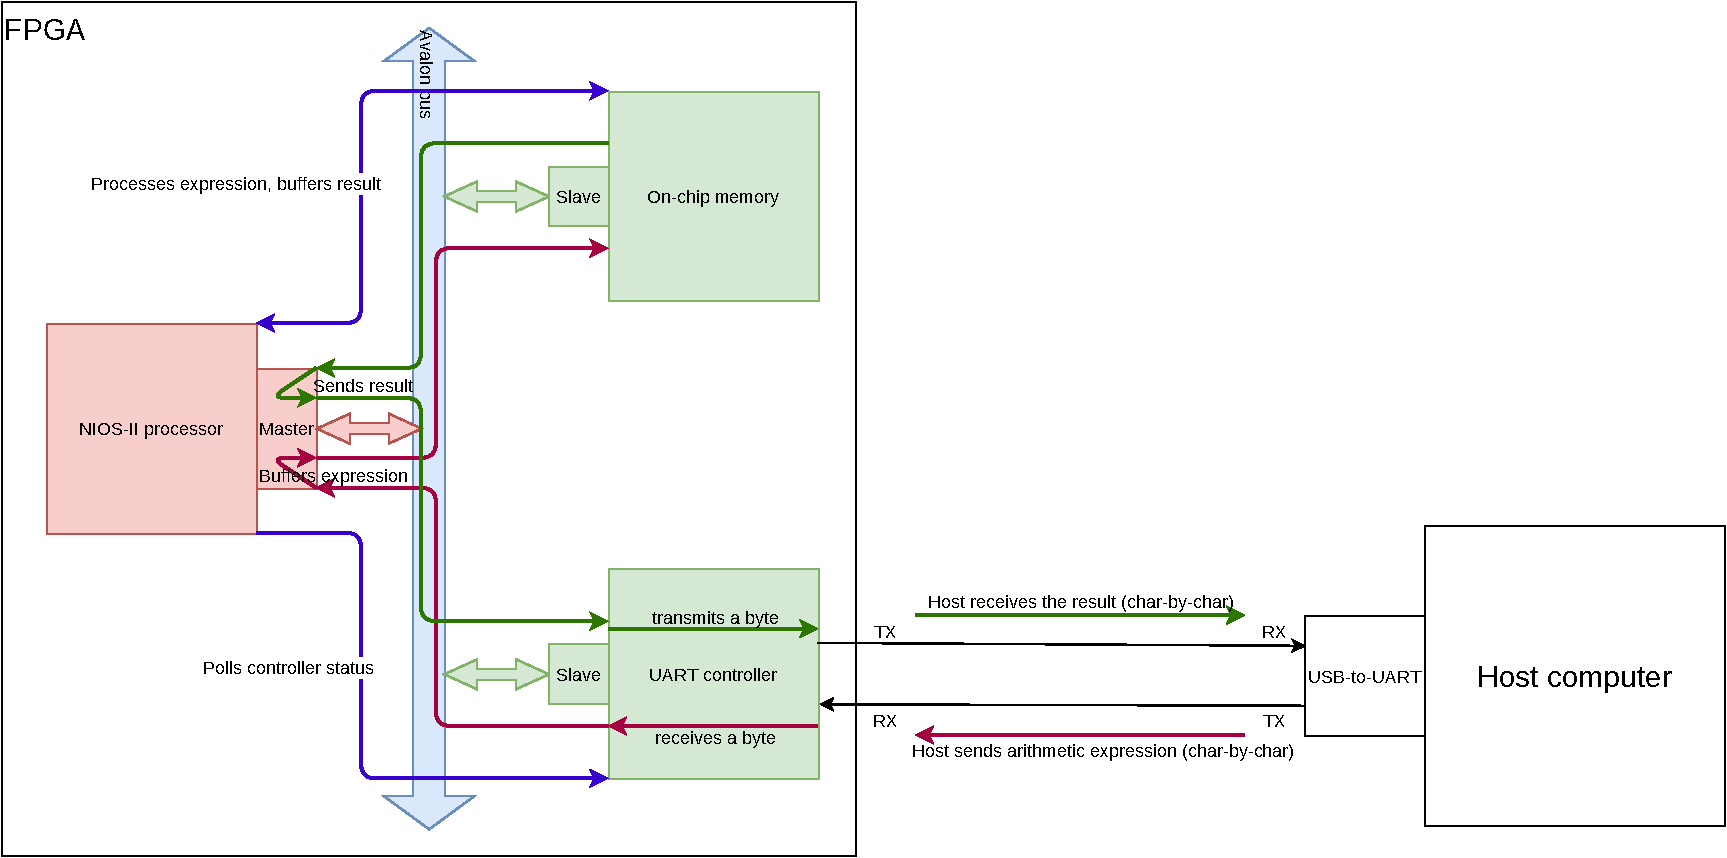
\includegraphics[width=\textwidth]{system}
	\caption{Overview of system architecture and operation}
	\label{fig:system}
\end{figure}

The standard operation of the application is the following:
\begin{enumerate}[nosep]
	\item The user types an arithmetic expression on the host terminal (used as an input device to the calculator).
	\item The host computer sends the sequence of bytes through the UART protocol to the controller on the FPGA.
	\item The UART controller receives these characters one-by-one, updating its status registers accordingly.
	\item The NIOS-II processor polls the controller to determine when new data has arrived, and buffers the received expression into memory.
	\item The processor parses the expression and prepares the response string, which is buffered into memory waiting for transmission.
	\item The processor polls the controller to determine when it is ready to transmit the next character, and sends the bytes one-by-one.
	\item The controller transmits each byte through the UART protocol to the host computer.
	\item The response is received by the host and displayed on the terminal (the output device of the calculator).
\end{enumerate}


\section{UART controller design}

In this section, we will describe the design and implementation of our custom UART controller. The goal is to create an Avalon memory-mapped slave peripheral, supporting configurable baud rate and parity, pollable status signals, and separate TX and RX buffers. The controller will then communicate using the UART protocol through a conduit consisting of a pair of TX/RX pins.

Some additional high-level design choices were made. The only supported data modes are:
\begin{itemize}[nosep]
	\item 8-bit data without parity and 1 stop bit (8N1 in minicom)
	\item 7-bit data with even parity and 1 stop bit (7E1)
	\item 7-bit data with odd parity and 1 stop bit (7O1).
\end{itemize}

In addition, a double-buffering system was chosen. This means that the controller doesn't have an internal FIFO; however it can store the next byte to transmit and the last byte received, while an active transmission and reception are going on.

\subsection{Programmable interface}

The physical interface of the peripheral is shown in figure \ref{fig:interface}. The controller has a clock and reset input, a memory-mapped slave interface, and a conduit for TX/RX.

\begin{figure}[h]
	\centering
	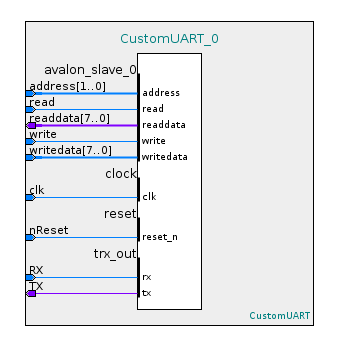
\includegraphics[width=.5\textwidth]{interface}
	\caption{Interface of the UART controller}
	\label{fig:interface}
\end{figure}

In table \ref{tab:map}, you can find the controller's register map.
We can see that the combined settings of clock divider (ranging from 1 to 128) and baud interval (ranging from 4 to 254 ticks/bit) allow -- assuming a \SI{50}{\mega\hertz} primary clock -- baud rates between 1.54 kBaud and 12.5 MBaud.

\begin{table}[h]
	\centering
	\begin{tabularx}{\linewidth}{|c|c|c|X|}
		\hline
		Address & Register & Bits & Description \\
		\hline
		\hline
		\multirow{6}{*}{0x00} & \multirow{6}{*}{CTRL A} & 0 & \textbf{RX available} (read-only): set when a new received byte is available. \\
		 & & 1 & \textbf{TX ready} (read-only): set when the controller is ready to accept the next byte for transmission. \\
		 & & 2 & \textbf{parity enable}: 1 to enable the parity bit (7-bit data + 1 parity bit), 0 to disable (8-bit data). \\
		 & & 3 & \textbf{parity odd}: 1 to use odd parity, 0 to use even parity (ignored if parity is disabled). \\
		 & & 4 - 6 & \textbf{clock divider}: $\log_2$ of the clock divider value, i.e. values between 0-7 are mapped to dividers 1-128. Transmission and reception logic (including the baud rate setting) are with respect to the slow clock. \\
		 & & 7 & unused, always returns 0. \\
		 \hline
		 0x01 & CTRL B & 0-7 & \textbf{baud rate}: represents the baud interval in terms of slow clock ticks per bit. Only values $\geq$ 4 are accepted. Since this setting must be even, the LSB is always 0. \\
		 \hline
		 0x02 & RX DATA & 0-7 & \textbf{RX data} (read-only): last correctly received byte. Reading from this register also clears the \textit{RXavailable} flag \\
		 \hline
		 0x03 & TX DATA & 0-7 & \textbf{TX data}: next byte to transmit. Writing to this register also clears the \textit{TXready} flag.\\
		 \hline
	\end{tabularx}
	\caption{Register map of the UART controller}
	\label{tab:map}
\end{table}

\subsection{Internal architecture}

\subsection{TX design}

\subsection{RX design}

\subsection{Timing of operations}

\subsection{Implementation details}


\section{Calculator software}

\subsection{UART driver}

\subsection{Main program}


\section{Operation \& results}


\section{Conclusion}


\end{document}